\documentclass{spaexp}
\major{物理学}
\name{梁伟德}
\grade{2017级}
\stuid{17353038}
\exptitle{E1\quad 高温超导实验}

\graphicspath{{img/}}

\begin{document}
    \maketitle
    
    \section{背景介绍}
    \section{实验原理}
        \subsection{实验目的}
        \subsection{超导}
        \subsection{降温与保温}
        \subsection{数据采集与分析}
            \subsubsection{电阻测量}
            实验中需要测量材料的电阻作为进入超导态的判断条件。测量接近0的小电阻需要四引线法\autoref{img:四引线测电阻电路原理图}。同时,还需考虑电阻由于不对称而引起的电势差:
            温差电势$V_T$,接触电势$V_C$。若使用直流电流进行测量,则有测量结果:$V_+ = IR + V_C + V_T$,为消除温差电势与接触电势,
            需要再进行一次反向电流的测量:$V_- = -IR + V_C + V_T$,可以得到:
            \begin{equation}
                R = \frac{V_+ - V_-}{2I}
            \end{equation}
            \begin{figure}
                \ct
                \caption{四引线测电阻电路原理图}
                \label{img:四引线测电阻电路原理图}
                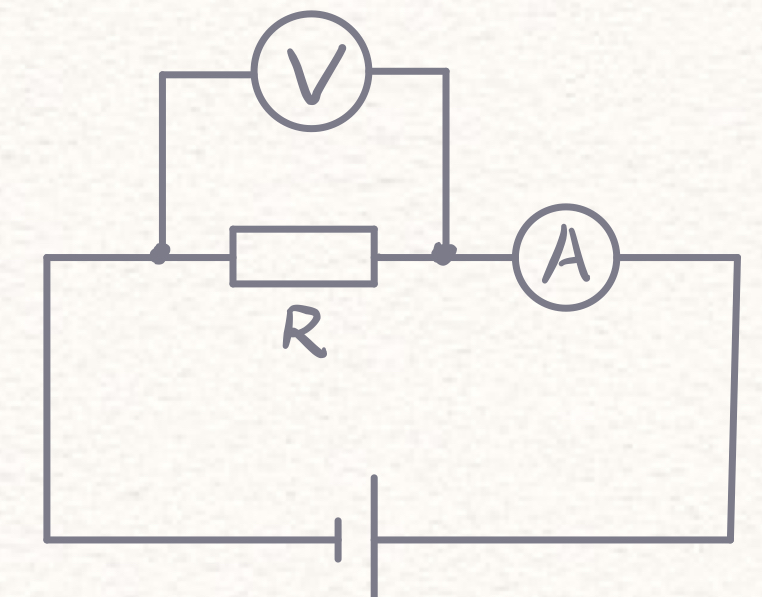
\includegraphics[width = 0.4\textwidth]{fourfoot.jpeg}
            \end{figure}

            实际测量时,变换两次电流方向分别测量,得到一个测量电阻值。在实验配备 IT6411S 可编程直流恒流源,可以通过计算机控制实现。\par

            为消除温差电势与接触电势,还可以使用{\bf{交流四引线测量法}},由交流电的特性可以直接排除直流电势的影响。使用锁相放大器测量弱小电阻是一个较好的选择。\autoref{img:锁相放大器实现交流四引线电阻测量}
            利用锁相功能不仅能排除直流噪声,还能排除其他高频噪声。\par

            使用交流电源对超导系统进行供电,讲电阻两侧用四引线接入锁相放大器的SIGNAL IN中则可以得到电阻两侧电势差,最终计算出超导材料的电阻。
            \begin{figure}
                \ct
                \caption{锁相放大器实现交流四引线电阻测量}
                \label{img:锁相放大器实现交流四引线电阻测量}
                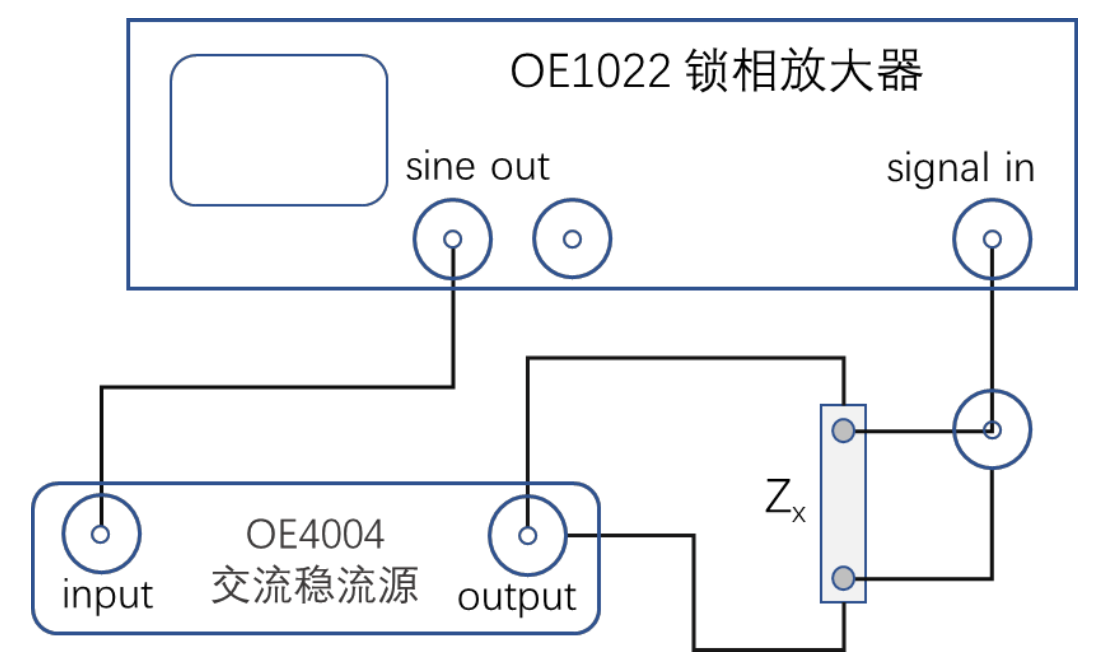
\includegraphics[width = 0.7\textwidth]{dcfourfoot.png}
            \end{figure}

            
    
    \section{实验方案}
        \subsection{液氮制冷获得超导态}
            \subsubsection{抽取真空}
                抽取真空需要用到较长时间,所以安装完恒温器后,可以先连接装置气路,开始抽真空,然后再进行其他仪器设备的连接。
                \begin{longtable}{@{*}p{0.7\textwidth}||p{0.3\textwidth}@{*}}
                    \caption{抽取真空操作步骤}\\
                    \hline\hline
                    \multicolumn{1}{@{*}>{\centering}p{0.7\textwidth}||}{\textbf{操作}}&\textbf{完成情况}\\
                    \hline\hline
                    连接真空抽口到真空泵之间的波纹管 & \\ \hline
                    通电前确认真空阀处于关闭状态(红色箭头,绿色阀与波纹管垂直)\autoref{img:真空阀实物俯视图}& \\ \hline
                    样品罩、机械泵等处的真空卡箍是拧紧的\autoref{img:真空阀实物俯视图} & \\ \hline
                    关闭真空阀门 & \\ \hline
                    开启真空泵(开关位于泵的侧面),计时2分钟 & \\ \hline
                    2分钟后缓慢拧开真空阀直至听见“呼噜”声为止 & \\ \hline
                    等待真空泵工作让“呼噜”声停止 & \\ \hline
                    缓慢拧开真空阀直至听见“呼噜”声为止 & \\ \hline
                    重复上述三个步骤直至真空阀完全打开 (绿色阀柄与波纹管平行)& \\ \hline
                    等待真空计示数小于5Pa(如果没有真空计,真空泵打开以后半个小时)& \\ \hline
                    关闭真空阀、关闭真空泵 & \\ \hline
                    在做上述步骤的时候,可安排另外同学同时进行下面的步骤 & \\ \hline
                \end{longtable}
                \begin{figure}
                    \ct
                    \caption{真空阀实物俯视图}
                    \label{img:真空阀实物俯视图}
                    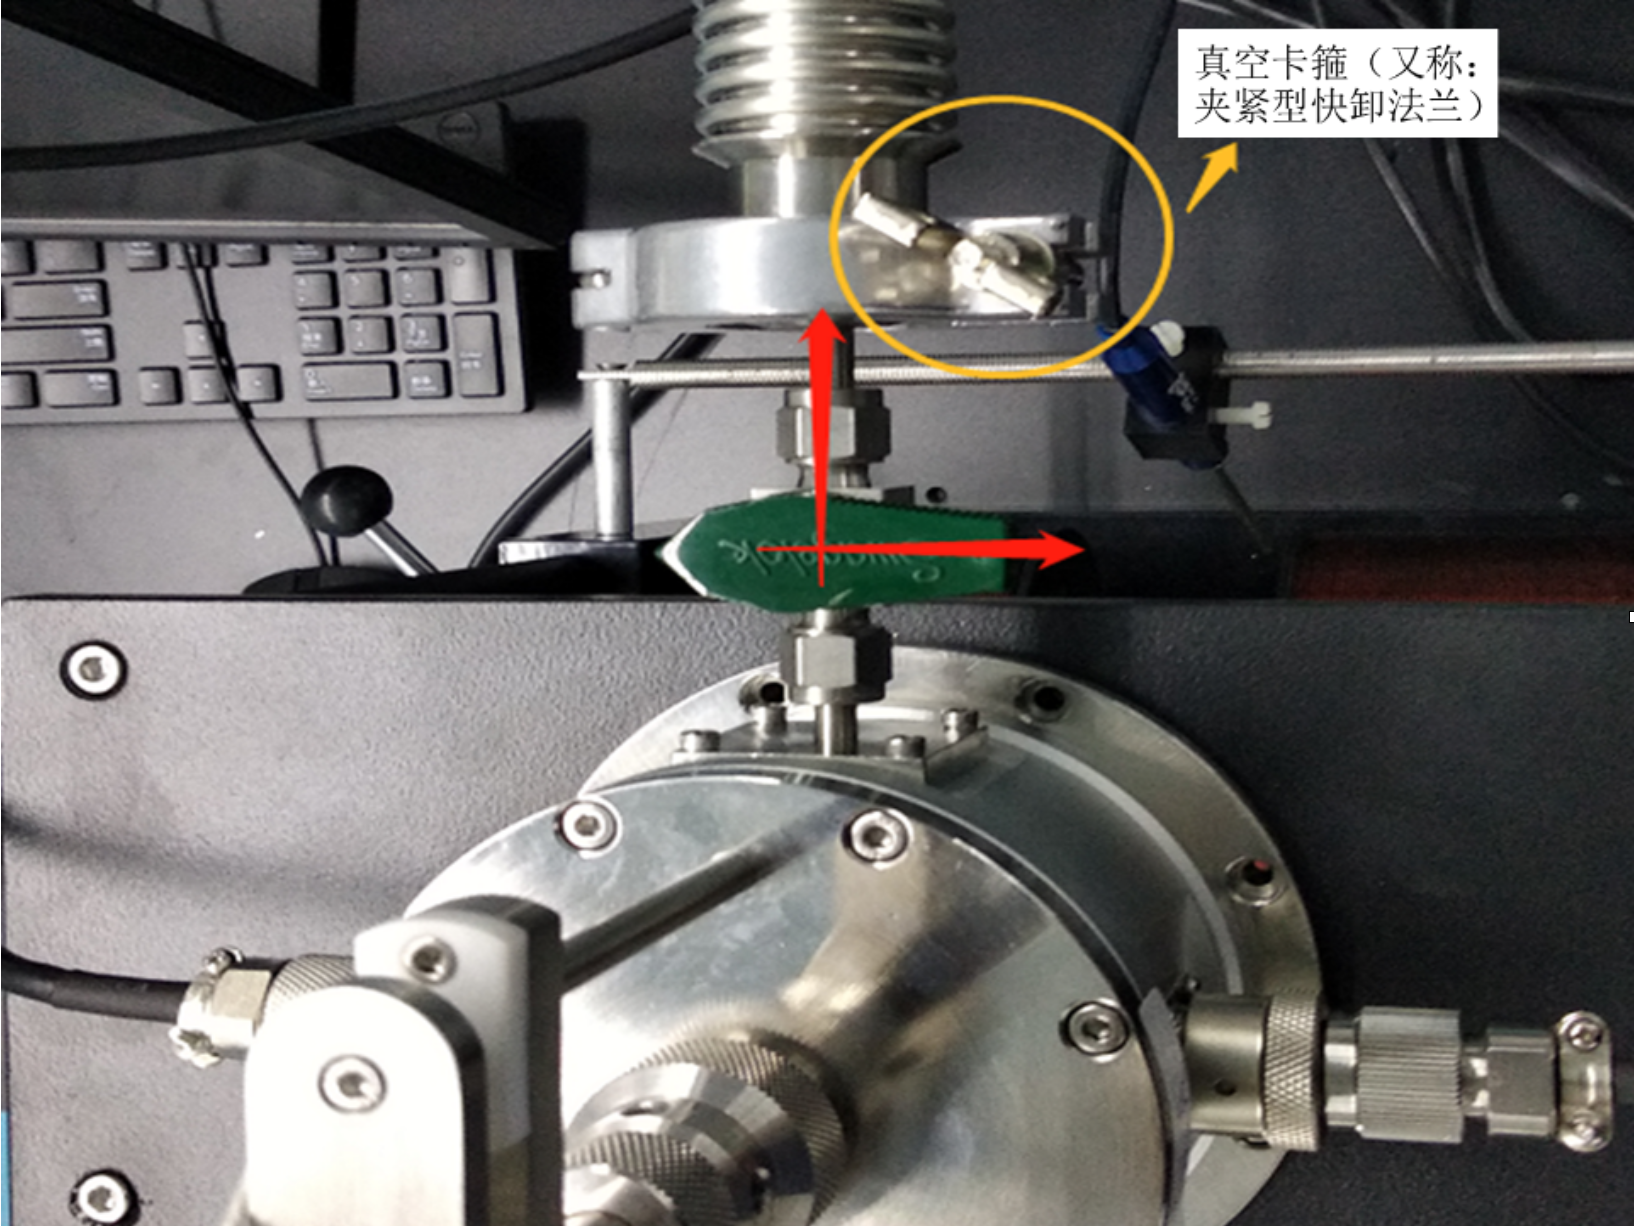
\includegraphics[width = 0.5\textwidth]{VacuumEntity.png}
                \end{figure}
                
            \subsubsection{设备电路连接}
                测量平台根据选择直流测量或交流测量而不同。
                \begin{longtable}{@{*}p{0.7\textwidth}||p{0.3\textwidth}@{*}}
                    \caption{设备电路连接操作步骤}\\
                    \hline\hline
                    \multicolumn{1}{@{*}>{\centering}p{0.7\textwidth}||}{\textbf{操作}}&\textbf{完成情况}\\
                    \hline\hline
                    使用BNC连接恒温器与控温仪(六芯) & \\ \hline
                    连接恒温器与NI等测量平台 (八芯)& \\ \hline
                    连接恒温器、测量平台到电脑 & \\ \hline
                \end{longtable}
                
                \begin{figure}
                    \ct
                    \caption{恒温器设备线路连接图}
                    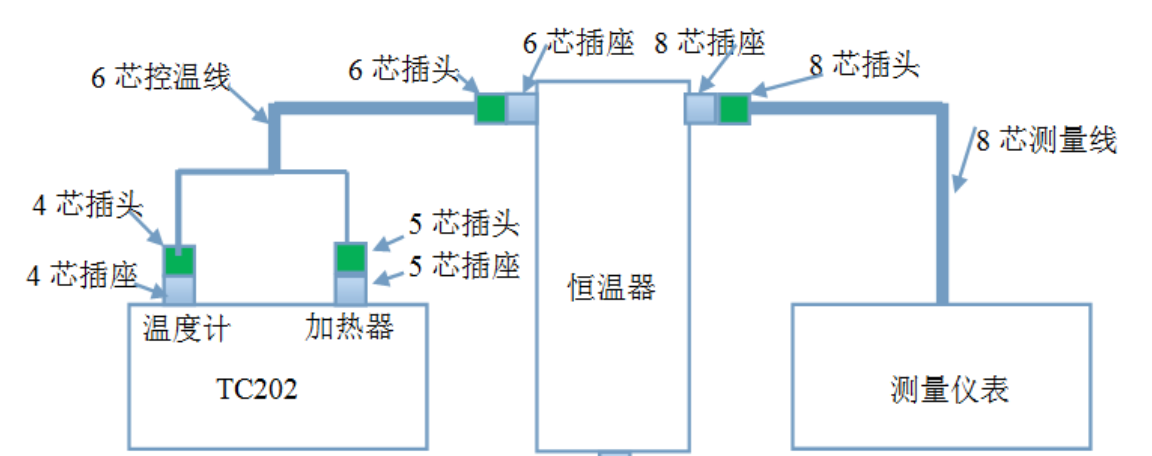
\includegraphics[width = 0.7\textwidth]{connection.png}
                \end{figure}

            \subsubsection{设备启动、预热}
                \begin{longtable}{@{*}p{0.7\textwidth}||p{0.3\textwidth}@{*}}
                    \caption{设备启动、预热操作步骤}\\
                    \hline\hline
                    \multicolumn{1}{@{*}>{\centering}p{0.7\textwidth}||}{\textbf{操作}}&\textbf{完成情况}\\
                    \hline\hline
                    打开NI机箱电源(前面板按钮) & \\ \hline
                    打开控温仪电源(前面板红色按钮) & \\ \hline
                    打开电磁铁电源(背后红色按钮,然后按前面板“power”长按3秒) & \\ \hline
                    打开OE4004电源预热 & \\ \hline
                    打开锁相放大器电源预热 & \\ \hline
                    打开普源数字多用表电源(先开后面板开关,再开前面板开关) & \\ \hline
                    打开电脑 & \\ \hline
                \end{longtable}
            
            \subsubsection{电脑程序与设备通讯}
                \begin{longtable}{@{*}p{0.7\textwidth}||p{0.3\textwidth}@{*}}
                    \caption{电脑程序与设备通讯操作步骤}\\
                    \hline\hline
                    \multicolumn{1}{@{*}>{\centering}p{0.7\textwidth}||}{\textbf{操作}}&\textbf{完成情况}\\
                    \hline\hline
                    打开电脑桌面LabView快捷方式“直流四引线测电阻”,检查设备连接 & \\ \hline
                \end{longtable}

            \subsubsection{液氮制冷}
                请熟悉液氮恒温器结构\autoref{img:液氮恒温器结构}与控温仪前面板\autoref{img:控温仪前面板}。控温过程控温仪负责控制加热速率,恒温器的中心塞控制制冷速率,两者合理调节
                才能或者较好的控温效果,请耐心调节。

                \begin{figure}
                    \ct
                    \caption{液氮恒温器结构}
                    \label{img:液氮恒温器结构}
                    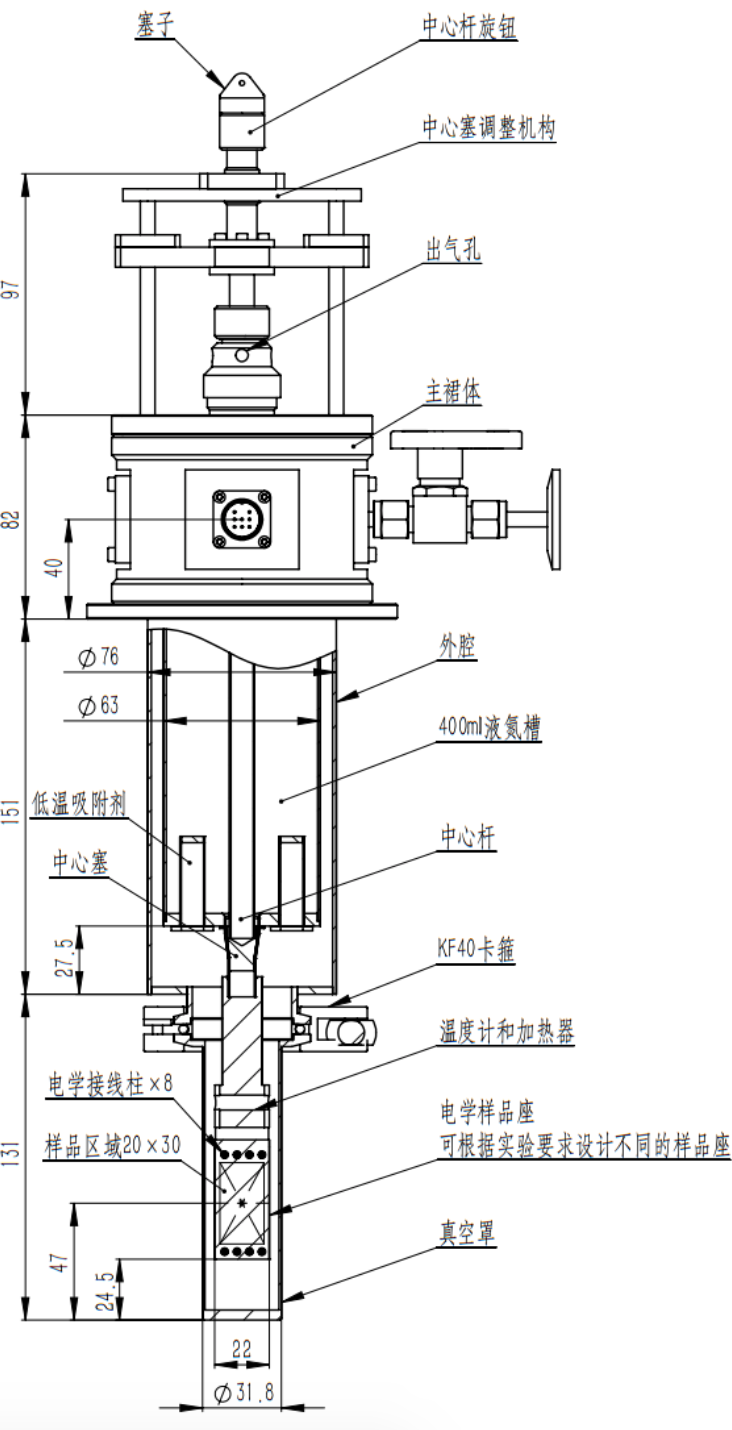
\includegraphics[width = 0.3\textwidth]{TempertureKeeper.png}
                \end{figure}
                \begin{figure}
                    \ct
                    \caption{控温仪前面板}
                    \label{img:控温仪前面板}
                    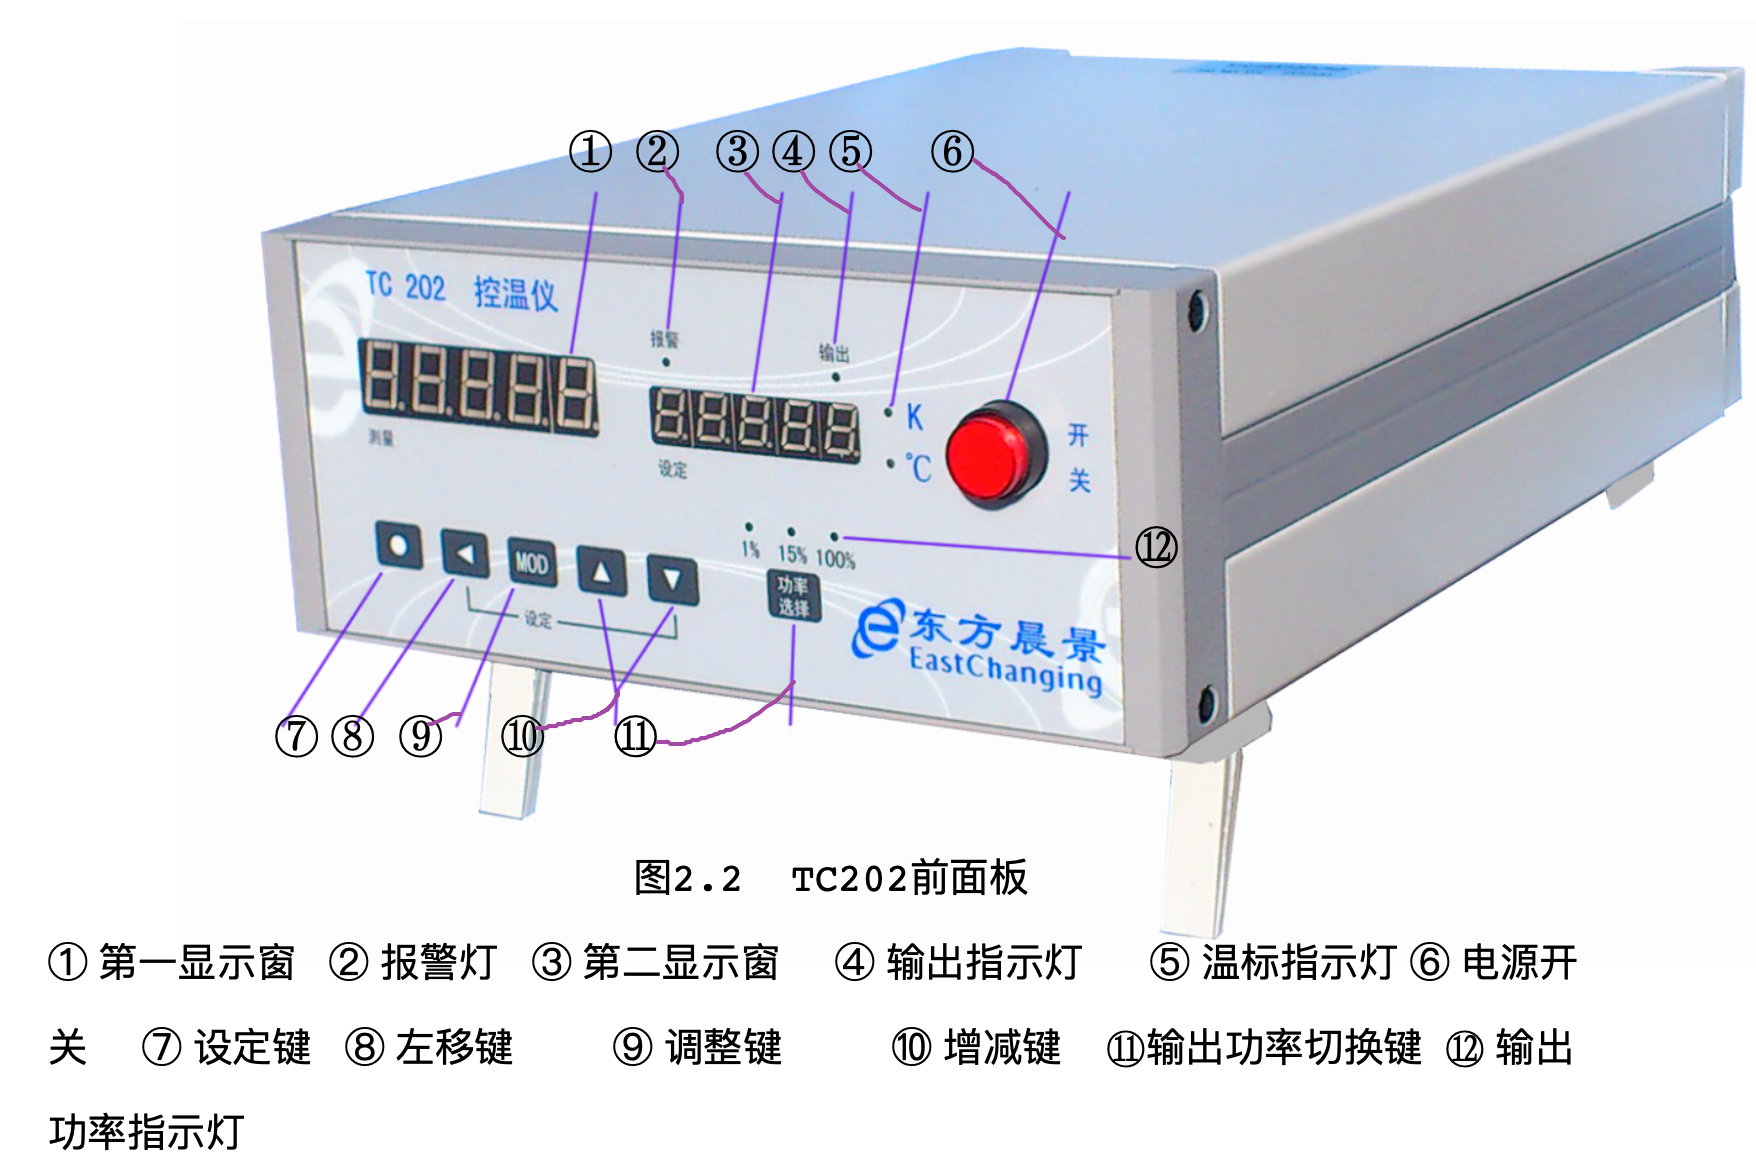
\includegraphics[width = 0.6\textwidth]{PIDFront.png}
                \end{figure}

                \begin{longtable}{@{*}p{0.7\textwidth}||p{0.3\textwidth}@{*}}
                    \caption{液氮制冷操作步骤}\\
                    \hline\hline
                    \multicolumn{1}{@{*}>{\centering}p{0.7\textwidth}||}{\textbf{操作}}&\textbf{完成情况}\\
                    \hline\hline
                    真空抽取结束,关闭真空阀真空泵 & \\ \hline
                    顺时针旋转“中心杆旋钮”至旋转比较费劲,此时中心塞完全关闭,液氮不会会样品制冷 & \\ \hline
                    逆时针旋转两圈“中心杆旋钮”,此时中心塞处于中间位置。 可根据所需降温速率调节旋钮 & \\ \hline
                    检查注液漏斗是否有水珠,保持注液漏斗干燥 & \\ \hline
                    取下恒温器顶部的塞子,检查注入口附近是否干燥。 & \\ \hline
                    插入注液漏斗,操作人员站在远离“出气孔”的一侧,缓慢的加入液氮,以防液氮溅射冻伤操作人员。直到液氮有少量溢出,表明液氮已经加注满 & \\ \hline
                    使用纱布包住“出气孔”,防止水汽进入恒温器内部 & \\ \hline

                    \multicolumn{2}{c}{\textbf{设定控温仪}} \\ \hline \hline
                    控温仪通过自检后,第一个显示屏显示实测温度,第二显示屏显示目标控温温度 & \\ \hline
                    按前面板左键(8号键),目标控温温度的低位开始闪烁,此时用上下键(10号键)调节数值,再按左键切换调节位。设置目标控温为:XX K等待闪烁停止完成调节 & \\ \hline
                    观察第一个窗口实测温度的变化,根据控温速率调节加热功率,按“功率选择”按钮选择功率。只有当“报警灯”不亮,“输出灯“与”功率指示灯“同时亮时,控温仪才会有加热输出 & \\ \hline
                    非必要时勿调节控温器参数,若要调节请仔细阅读《控温仪TC202说明书》 & \\ \hline
                \end{longtable}
                
            \subsubsection{数据测量}
                需要通过测量样品的电阻或抗磁率,找到样品进入超导态的\textbf{转变温度}。
                \begin{longtable}{@{*}p{0.7\textwidth}||p{0.3\textwidth}@{*}}
                    \caption{第一次数据测量操作步骤}\\
                    \hline\hline
                    \multicolumn{1}{@{*}>{\centering}p{0.7\textwidth}||}{\textbf{操作}}&\textbf{完成情况}\\
                    \hline\hline
                    根据测量方案利用计算机进行测量值采集,输出测量记录并保存,记录文件名: & \\ \hline
                \end{longtable}

            \subsubsection{实验结束}
                测量完所需数据后,若需要拆开液氮恒温器改变实验则需要按照操作步骤结束恒温器的工作状态,不可暴力拆除。
                若改变的实验条件不需要拆开液氮恒温器如:加入磁场。则不需要结束恒温器工作状态。
                \begin{longtable}{@{*}p{0.7\textwidth}||p{0.3\textwidth}@{*}}
                    \caption{结束实验操作步骤}\\
                    \hline\hline
                    \multicolumn{1}{@{*}>{\centering}p{0.7\textwidth}||}{\textbf{操作}}&\textbf{完成情况}\\
                    \hline\hline
                    确定真空阀关闭状态,关闭真空泵 & \\ \hline
                    使用控温仪加热到290K稳定后,关闭控温仪及其他仪器 & \\ \hline
                    把所有连接线拆除,盖上恒温器塞子 & \\ \hline
                \end{longtable}
    \section{分析与讨论}
        \subsection{实验思考题}

\end{document}